\chapter{Sequences \& Series of Functions}
For a metric space $X$ and a sequence of functions $f_n:X\to\reals$, we want to define what it means for the sequence to `approach' a function, i.e., what is meant by $f_n\to f$ (or $\sum^\infty_{n=1}f_n=f$) on $X$.

\section{Point-wise Convergence.}
We say $f_n\to f$ \emph{point-wise} on $E\subset X$ if $f_n(x)\to f(x)\,\forall x\in E$.
Similarly, $\sum f_n\to f\iff \sum f_n(x)\to f(x)\,\forall x\in E$.

This definition is intuitive, however, has little use because of several drawbacks.

\subsection{Point-wise convergence destroys continuity:}
Let $f_n(x)=x^n,x\in[0,1]$.
Note that $f_n(x)\to 0,x\in[0,1)$ and $f(1) = 1$.
A graphical proof of this is shown in Fig. \ref{fig:ptwiseCont}.
\begin{figure}[!ht]
    \centering
    \scalebox{0.6}{


\tikzset{every picture/.style={line width=0.75pt}} %set default line width to 0.75pt        

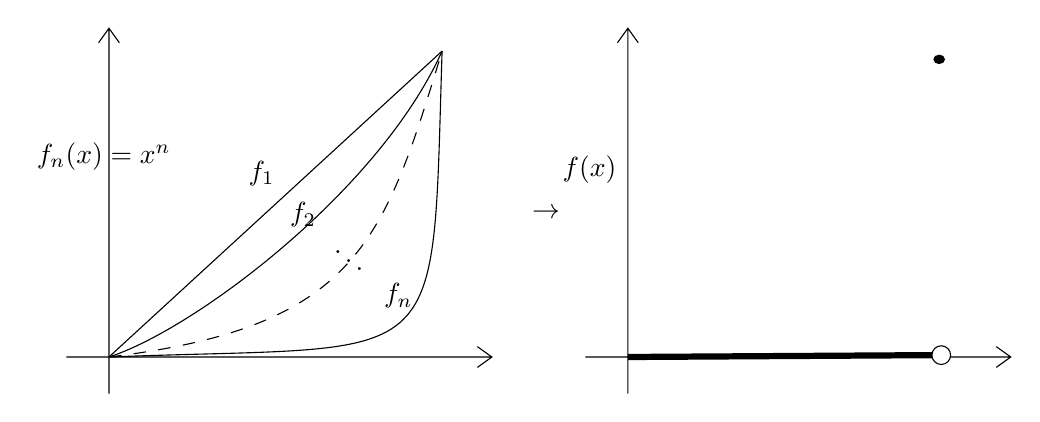
\begin{tikzpicture}[x=0.75pt,y=0.75pt,yscale=-1,xscale=1]
%uncomment if require: \path (0,478); %set diagram left start at 0, and has height of 478

%Shape: Axis 2D [id:dp905814360049316] 
\draw  (72,381.4) -- (277,381.4)(92.5,223) -- (92.5,399) (270,376.4) -- (277,381.4) -- (270,386.4) (87.5,230) -- (92.5,223) -- (97.5,230)  ;
%Shape: Axis 2D [id:dp0627612849597261] 
\draw  (322,381.4) -- (527,381.4)(342.5,223) -- (342.5,399) (520,376.4) -- (527,381.4) -- (520,386.4) (337.5,230) -- (342.5,223) -- (347.5,230)  ;
%Straight Lines [id:da2673655934702972] 
\draw    (92.5,381.4) -- (253,234) ;


%Straight Lines [id:da766634506285276] 
\draw [line width=2.25]    (342.5,381.4) -- (489,380.5) ;


%Shape: Ellipse [id:dp7944840513243177] 
\draw  [fill={rgb, 255:red, 0; green, 0; blue, 0 }  ,fill opacity=1 ] (490,238) .. controls (490,239.1) and (491.12,240) .. (492.5,240) .. controls (493.88,240) and (495,239.1) .. (495,238) .. controls (495,236.9) and (493.88,236) .. (492.5,236) .. controls (491.12,236) and (490,236.9) .. (490,238) -- cycle ;
%Shape: Circle [id:dp9726229856614172] 
\draw  [fill={rgb, 255:red, 255; green, 255; blue, 255 }  ,fill opacity=1 ] (489,380.5) .. controls (489,378.01) and (491.01,376) .. (493.5,376) .. controls (495.99,376) and (498,378.01) .. (498,380.5) .. controls (498,382.99) and (495.99,385) .. (493.5,385) .. controls (491.01,385) and (489,382.99) .. (489,380.5) -- cycle ;
%Curve Lines [id:da8879947029325801] 
\draw    (92.5,381.4) .. controls (134,368) and (223,301) .. (253,234) ;


%Curve Lines [id:da5540476052003762] 
\draw  [dash pattern={on 4.5pt off 4.5pt}]  (92.5,381.4) .. controls (212,367) and (225,326) .. (253,234) ;


%Curve Lines [id:da7987092769906381] 
\draw    (92.5,381.4) .. controls (257,375) and (248,393) .. (253,234) ;





% Text Node
\draw (90,285) node   {$f_{n}( x) =x^{n}$};
% Text Node
\draw (303,312) node   {$\rightarrow $};
% Text Node
\draw (166,293) node   {$f_{1}$};
% Text Node
\draw (186,313) node   {$f_{2}$};
% Text Node
\draw (232,352) node   {$f_{n}$};
% Text Node
\draw (208,331) node   {$\ddots $};
% Text Node
\draw (324,291) node   {$f( x)$};


\end{tikzpicture}
}
    \caption{$f_n$'s are continuous $\forall n$ but their limit is not}
    \label{fig:ptwiseCont}
\end{figure}

\subsection{Point-wise convergence destroys integral:}
Let $f_n(x)=(2n+2)x(1-x^2)^n$ on $[0,1]$ and $f_n(0)=f_n(1)=0$.
\vspace{-1.5in}
\begin{figure}[!ht]
    \centering
    \scalebox{0.6}{


\tikzset{every picture/.style={line width=0.75pt}} %set default line width to 0.75pt        

\begin{tikzpicture}[x=0.75pt,y=0.75pt,yscale=-1,xscale=1]
%uncomment if require: \path (0,478); %set diagram left start at 0, and has height of 478

%Shape: Axis 2D [id:dp5116854562026876] 
\draw  (224,201.4) -- (429,201.4)(244.5,43) -- (244.5,219) (422,196.4) -- (429,201.4) -- (422,206.4) (239.5,50) -- (244.5,43) -- (249.5,50)  ;
%Shape: Axis 2D [id:dp9643251095140839] 
\draw  (445,201.4) -- (650,201.4)(465.5,43) -- (465.5,219) (643,196.4) -- (650,201.4) -- (643,206.4) (460.5,50) -- (465.5,43) -- (470.5,50)  ;
%Curve Lines [id:da26994130810027617] 
\draw    (244.5,201.4) .. controls (261,-4) and (348,198) .. (409,202) ;


%Curve Lines [id:da8291195950058514] 
\draw    (244.5,201.4) .. controls (255,-81) and (297,199) .. (409,202) ;


%Curve Lines [id:da809996449988654] 
\draw    (244.5,201.4) .. controls (259,-190) and (235,193) .. (409,202) ;


%Straight Lines [id:da12190932696161982] 
\draw [line width=2.25]    (625,201) -- (465.5,201.4) ;




% Text Node
\draw (446,98) node   {$\rightarrow $};
% Text Node
\draw (224,70) node   {$f_{n}( x)$};
% Text Node
\draw (448,72) node   {$f( x)$};
% Text Node
\draw (337,126) node   {$f_{1}$};
% Text Node
\draw (293,80) node   {$f_{2}$};
% Text Node
\draw (273,21) node   {$f_{n}$};


\end{tikzpicture}
}
    \caption{$f_n$'s are continuous $\forall n$ but their limit is not}
    \label{fig:ptwiseInt}
\end{figure}

Note from Fig. \ref{fig:ptwiseInt} that $f_n\to 0\implies \int^1_0 f = 0$, but $\int^1_0 f=1$.
Therefore, point-wise convergence does not preserve the value of the integral.

\subsection{Point-wise convergence destroys integrability:}
Let $f_N(x)=1$ if $x=m/n,\,n\leq N$ and $0$ otherwise.
Since $f_N$ has finitely many discontinuities on $[0,1]\implies f_N\in\mathcal{R}$.
However, $\lim_{N\to\infty f_N\to}$ Dirichlet's function, which is not integrable.

Therefore, we need to come up with a better criterion for convergence of sequences of functions that preserve these properties.

\section{Uniform Convergence.}
\begin{definition}[Uniform Convergence]
We say $f_n\to f$ \emph{uniformly} on $E\subset X$ if for any $\varepsilon>0\,\exists N_\varepsilon>0$ such that $\abs{f_n(x)-f(x)}<\varepsilon$ if $n\geq N_\varepsilon$ for \emph{any} $x\in E$.
\end{definition}
\begin{definition}[Uniform norm]
$f_n\to f$ uniformly on $E\iff\sup_E \abs{f_n-f}\to 0$.
Then we can define the uniform norm as $\norm{f_n-f}\coloneqq \sup_E \abs{f_n-f}$.
\end{definition}
In other words, we claim uniform convergence w.r.t. to this newly defined distance approaching zero.

\subsection{Cauchy criterion for Uniform Convergence.}
$f_n$ is a uniformly convergent sequence of functions on $E$ if for any $\varepsilon>0,\exists N_\varepsilon>0$ such that $\abs{f_n(x)-f_m(x)}<\varepsilon$ if $n,m>N_\varepsilon,\,\forall x\in E$.

Similarly, for series convergence, $\sum f_n(x)$ converges uniformly on $E\iff$ for any $\varepsilon>0,\,\exists N_\varepsilon>0$ such that $\abs{\sum^m_{k=n}f_k(x)}\leq \varepsilon$ if $m\geq n\geq N_\varepsilon$. 

\begin{theorem}[Weierstrass M-test]
Suppose $\exists M_n\geq 0$ such that $\sum^\infty_0 M_n$ is finite and $\abs{f_x(x)}\leq M_n,n\geq n_0\,\forall x\in E\implies \sum f_n(x)$ converges uniformly on $E$.
\end{theorem}

\subsection{Uniform convergence \& continuity.}
Let $E\subset X$ and $c$ a limit point of $E$.
Let $f_n:E\to \reals$ and let $A_n=\lim_{x\to c} f_n(x)$ exist.
If $f_n\to f$ uniformly on $E$, then $A=\lim_{x\to c}f(x)$ exists and $A=\lim_{n\to\infty} A_n$, i.e.,
\begin{equation*}
\lim_{n\to\infty} \underbrace{\lim_{x\to c}f_n(x)}_{A_n} = \lim_{x\to c}\underbrace{\lim_{n\to\infty} f_n(x)}_{f(x)}
\end{equation*}
\begin{remark}
This swapping of limits is allowed only for uniform convergence. As we saw in the previous section, point-wise convergence destroys preservation of limits.\\
\emph{Corollary:} If $f_n\to f$ uniformly on $E$ and $f_n$'s are continuous on $E\implies f(x)$ is continuous on $E$.
\end{remark}

\subsection{Uniform convergence \& integrals.}
Let $f_n:[a,b]\to\reals,f_n\in\mathcal{R}(\alpha)$ w.r.t some $\alpha$ on $[a,b]$.
If $f_n\to f$ uniformly on $[a,b]\implies f\in \mathcal{R}(\alpha)$ on $[a,b]$ and 
\begin{equation*}
\int^b_a fd\alpha = \lim_{n\to \infty} \int^b_a f_n d\alpha
\end{equation*}

\subsection{Uniform convergence \& differentiation.}
Suppose $f_n:(a,b)\to\reals$ be differentiable on $(a,b)$ and if $f_n\to f$ uniformly, then 
\begin{equation*}
\lim_{n\to\infty} f'_n(x) = \left(\lim_{n\to\infty}f_n(x)\right)'
\end{equation*}

\section{Equicontinuous Families.}

\section{Stone-Weierstrass theorem.}